\subsection{Login}
\label{sub:login}

Det første modul der interageres med, er loginmodulet, som har til formål at validere, og videresende brugeren til programmets hovedfunktioner.

\subsubsection{Funktionalitet}
\label{ssub:login_funktionalitet}

Loginmodulet har det primære ansvar for at angive adgangsniveauer, og sikre databeskyttelse. Fra loginmodulet kan man vælge at oprette sig som ny gæst, eller logge ind i systemet. Hvis brugeren vælger at oprette sig som ny gæst, så vil brugeren blive sendt til et separat modul.

\subsubsection{Implementation}
\label{ssub:login_implementation}

\begin{figure}
  \centering
  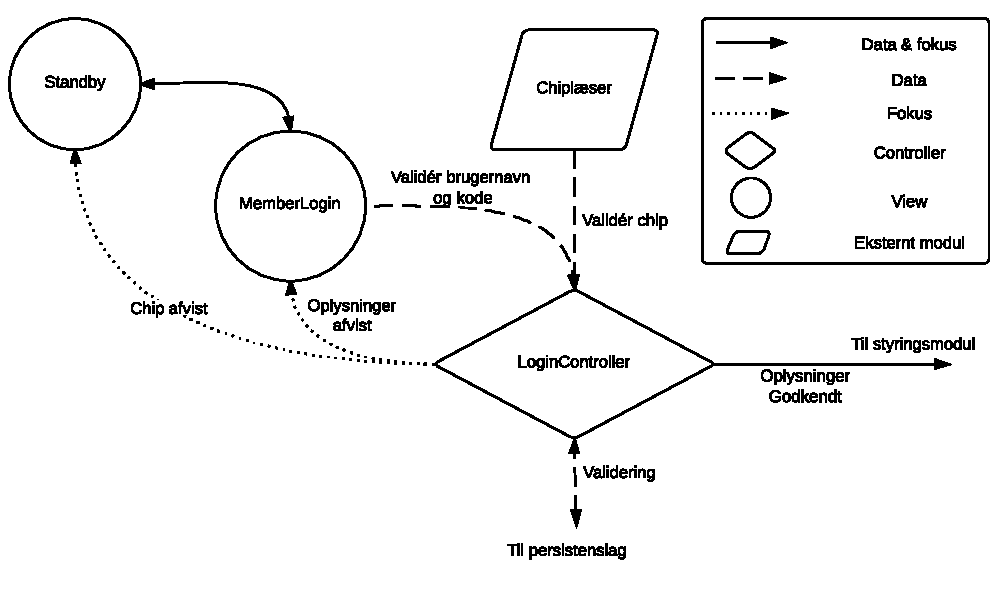
\includegraphics[width=\textwidth]{login-diagram.pdf}
  \caption{Dette er bare noget filler tekst.}
\end{figure}

\sinote{standby og element skal være mere beskrivende}

Loginmodulet består af et standby- og memberlogin-modul, et eksternt chiplæser-modul samt en loginController.
LoginControlleren modtager data fra memberlogin- og chiplæser-modulerne og kommunikere med persistenslaget hvor den validere dataen i forhold til det eksisterende data. Hvis chippen eller loginoplysningerne bliver afvist, sender controlleren brugeren tilbage til standby-modulet hvorefter brugerens input afventes.
Standby-modulet, alt efter brugerens input, sender brugeren videre til enten memberlogin-modulet eller guestcreation(REFERENCE TIL AFSNIT OMKRING GUESTCREATOR). Memberlogin-modulet sender den data brugeren indtastede til loginControlleren. Alt efter loginControllerens output, vil brugeren blive videre sendt eller returneret til memberlogin.


%Loginmodulet består af et standby-, chiplogin-, guestcreator-, medlemslogin-, validering- og videresendingselement. Standby-elementetet står for at sende brugeren til enten chip-, guestcreator- eller medlemlogin-elementet. Chip- og medlemslogin benytter begge validerings-modulet, som valider brugerens input, henholdsvis chipkortet og et medlems loginoplysninger. Dernæst aktiveres videresendings-modulet. Videresendingsmodulet sender enten brugeren ind i programmet eller tilbage til standby-modulet, afhængig af validerings-modulets output.

%Loginmodulet består af et standby-, medlemslogin-, validerings-, samt videresendings-element.

%Standby-elementet er udgangspunktet for al interaktion med programmet, og har henvisninger til hvordan brugeren anvender programmet. 

%Fra standby-elementet kan brugeren vælge at gå til medlemslogin-elementet, hvor en bruger der er medlem kan logge sig ind med sit medlemsnummer, og et kodeord. Herfra bør man også kunne vende tilbage til standby-elementet, i tilfælde af fejl.

%Alternativt kan brugeren indsætte et chipkort fra standby-elementet, og så sender standby-elementet brugeren direkte til validerings-elementet.

%Medlemsnummeret og kodeordet bliver videresendt til validerings-elementet, som krydstjekker informationerne via databasemodulet. Validerings-elementet videresender herefter en boolsk statusmelding, samt en brugerprofil fra databasen til videresendings-elementet.


%Videresendings-elementet tjekker status meldingen. Hvis meldingen er falsk, sender den brugeren tilbage til enten medlemslogin eller standby, med en passende fejlmelding. Hvis valideringen gik godt, så videresendes brugeren til styringsmodulet.
